%%% api - conceito e funcionalidade
\begin{frame}{API - Conceptualização e Funcionalidades}

\vspace*{-4em}

\begin{itemize}
	\item Entidades:
	\begin{itemize}
		\item \textbf{Voluntário}: indivíduo participante da ação;
		\item \textbf{Organização}: entidade que organiza ação;
		\item \textbf{Evento}: ação de voluntariado;
		\item \textbf{\textit{Post}}: meio de interação entre utilizadores.
	\end{itemize}

	\vspace*{1em}

	\item Funcionalidades:
	\begin{itemize}
		\item adicionar e alterar entidades;
		\item assegurar interação entre utilizadores;
		\item permitir que organizações possam verificar e obter contatos de voluntários interessados.
	\end{itemize}
\end{itemize}

\end{frame}

%%% api - arquitetura
\begin{frame}{API - Arquitetura}

\vspace*{-3em}

\begin{itemize}
	\item \textbf{Controladores}: definem \textit{endpoints} e lidam com pedidos HTTPS;
	\item \textbf{Serviços}: implementam a lógica de negócio;
	\item \textbf{Repositórios}: interagem com a base de dados.
\end{itemize}

\centering
\scalebox{0.20}{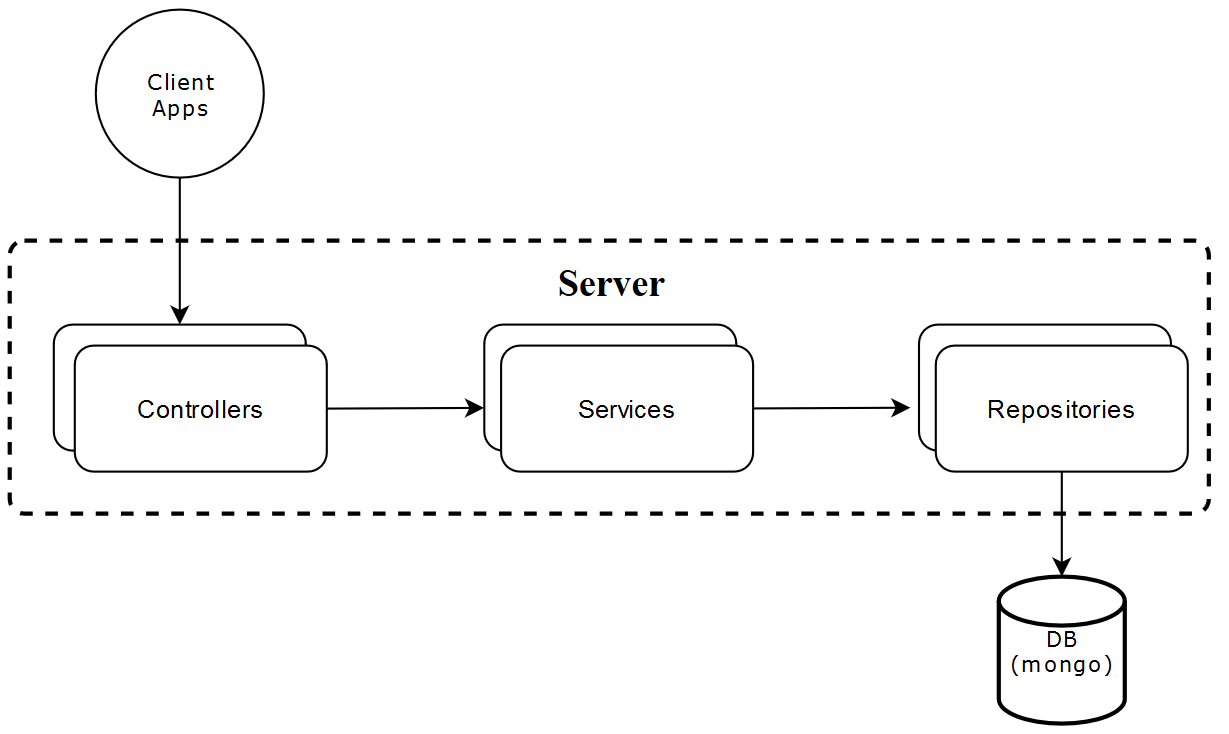
\includegraphics{Figures/api_architecture}}\\
{\small Arquitetura da API.}

\end{frame}